\chapter{Analyse et conception}
\addcontentsline{toc}{chapter}{Analyse et conception}
\markboth{Analyse et conception}{Analyse et conception}
\label{chap:analyseEtConception}
% section starts from 1 
%\minitoc

\section{Introduction}
Afin de pouvoir implémentées les fonctionnalités recensées au début de ce projet, nous
s'intéressons dans ce chapitre à l'étude conceptuelle de notre application. C'est une phase de spécification et de modélisation conceptuelle basée sur le langage UML à travers les diagrammes de cas d'utilisation, les diagrammes de séquences et classes. Ceci nous permet de tracer une meilleure stratégie d'implémentation des besoins fonctionnels tout en respectant les contraintes identifiées. Ensuite, nous exposerons les besoins non fonctionnels ainsi que notre backlog de produit.

\section{Analyse}
Dans cette phase d'analyse nous allons identifier les acteurs de notre application et les
différents besoins fonctionnels et non fonctionnels.

\subsection{Identifications des acteurs}
Un utilisateur est une entité extérieure au système de modélisation qui représente et
interagit directement avec une personne, un appareil. Chaque acteur dispose d'un ensemble
d'actions correspondant à la fonction dont il a besoin. Dans notre projet

L'application « Elise » Mobile fait intervenir plusierus acteurs comme le montre le tableau ci-après.

\begin{table}[h]
\setlength\tabcolsep{3pt}
\centering
\begin{tabularx}{\textwidth}{|c|L|}
\hline
Acteur & Rôles \\ 
\hline
\textbf{Collaborateur} & Accéde aux documents qui lui sont partagés, peut les modifier et les partager selon les tâches qui lui sont assignées \\ \hline
\textbf{Secrétaire} & Même rôle que le collaborateur avec en plus l'accès aux documents partagés par les autres de son service et les documents partagés par les autres services des collaborateurs \\ \hline
\textbf{Chef de service} & Même rôle que le secrétaire avec en plus l'accès aux documents partagés par les autres services subalternes \\ \hline
\end{tabularx}
\caption{Acteurs de l'application}
\label{tab:acteurs}
\end{table}



% note
\begin{small}
  Ces rôles/droits sont définis et appliqués par défaut par le système. Il est possible de les modifier selon les besoins spécifiques du client.
\end{small}

\subsection{Spécifications des besoins fonctionnels}
Notre application est desinée aux utilisateurs suivants : les collaborateurs, les secrétaires et les chefs de service. Chacun d'eux dispose d'un ensemble d'actions correspondant à la fonction dont il a besoin.

\subsubsection{Besoins fonctionnels des collaborateurs}
\begin{itemize}
% \item \textbf{Authentification} : L'utilisateur doit pouvoir s'authentifier à l'application pour pouvoir accéder à ses documents.
% \item \textbf{Consultation de profil} : L'utilisateur doit pouvoir consulter son profil.
% \item \textbf{Modification de profil} : L'utilisateur doit pouvoir modifier son profil.
% \item \textbf{Declaration d'absence} : L'utilisateur doit pouvoir déclarer son absence.
% \item \textbf{Annulation d'absence} : L'utilisateur doit pouvoir annuler son absence.
% \item \textbf{Affectation de delegé} : L'utilisateur doit pouvoir affecter un ou plusieurs délégué(s) pour le remplacer en cas d'absence.
% \item \textbf{Suppression de delegé} : L'utilisateur doit pouvoir supprimer un ou plusieurs délégué(s) affecté(s).
% \item \textbf{Recherche d'un utilisateur/service} : L'utilisateur doit pouvoir rechercher un utilisateur ou un service.
% \item \textbf{Reception de notification} : L'utilisateur doit pouvoir recevoir une notification de rappel.
% \item \textbf{Désactivation de notification} : L'utilisateur doit pouvoir désactiver les notifications.
% \item \textbf{Consulter espace de travail utilisateur} : L'utilisateur doit pouvoir consulter son espace de travail.
% \item \textbf{Consulter espace de travail personnalisé} : L'utilisateur doit pouvoir consulter son espace de travail personnalisé.
% \item \textbf{Supprimer espace de travail personnalisé} : L'utilisateur doit pouvoir supprimer son espace de travail personnalisé.
% \item \textbf{Modifier espace de travail personnalisé} : L'utilisateur doit pouvoir modifier son espace de travail personnalisé.
% \item \textbf{Ajouter un espace de travail personnalisé} : L'utilisateur doit pouvoir ajouter un espace de travail personnalisé.
% \item \textbf{Accéder aux espaces de travail de ses différents services} : L'utilisateur doit pouvoir accéder aux espaces de travail de ses différents services.
% \item \textbf{Consulter tableau de bord partagé et personnel} : L'utilisateur doit pouvoir consulter son tableau de bord partagé et personnel.
% \item \textbf{Consulter les widgets du tableau de bord personnel} : L'utilisateur doit pouvoir consulter les widgets de son tableau de bord personnel.
% \item \textbf{Ajouter un widget dans le tableau de bord personnel} : L'utilisateur doit pouvoir ajouter un widget dans son tableau de bord personnel.
% \item \textbf{Supprimer un widget dans le tableau de bord personnel} : L'utilisateur doit pouvoir supprimer un widget dans son tableau de bord personnel.
% \item \textbf{Configurer un widget du tableau de bord personnel} : L'utilisateur doit pouvoir configurer un widget de son tableau de bord personnel.
% \item \textbf{Ajouter un tableau de bord personnel} : L'utilisateur doit pouvoir ajouter un tableau de bord personnel.
% \item \textbf{Supprimer un tableau de bord personnel} : L'utilisateur doit pouvoir supprimer un tableau de bord personnel.
% \item \textbf{Modifier un tableau de bord personnel} : L'utilisateur doit pouvoir modifier un tableau de bord personnel.
% \item \textbf{Rechercher un document selon le filtre} : L'utilisateur doit pouvoir rechercher un document selon le filtre.
% \item \textbf{Accéder à l'ensemble de ses tâches} : L'utilisateur doit pouvoir accéder à l'ensemble de ses tâches.
% \item \textbf{Superviser son processus métier} : L'utilisateur doit pouvoir superviser son processus métier.
% \item \textbf{Démarrer une tâche dans un document} : L'utilisateur doit pouvoir démarrer une tâche dans un document.
% \item \textbf{Modifier informations d'un document} : L'utilisateur doit pouvoir modifier les informations d'un document.
% \item \textbf{Consulter les fichiers d'un document} : L'utilisateur doit pouvoir consulter les fichiers d'un document.
% \item \textbf{Supprimer un fichier d'un document} : L'utilisateur doit pouvoir supprimer un fichier d'un document.
% \item \textbf{Ajouter un fichier à un document} : L'utilisateur doit pouvoir ajouter un fichier à un document.
% \item \textbf{Consulter l'historique d'un document} : L'utilisateur doit pouvoir consulter l'historique d'un document.
% \item \textbf{Consulter les tâches d'un document} : L'utilisateur doit pouvoir consulter les tâches d'un document.
% \item \textbf{Supprimer une tâche d'un document} : L'utilisateur doit pouvoir supprimer une tâche d'un document.
% \item \textbf{Ajouter une tâche à un document} : L'utilisateur doit pouvoir ajouter une tâche à un document.
% \item \textbf{Consulter l'historique d'une tâche} : L'utilisateur doit pouvoir consulter l'historique d'une tâche.
% \item \textbf{Consulter les signatures} : L'utilisateur doit pouvoir consulter les signatures.
% \item \textbf{Ajouter une signature} : L'utilisateur doit pouvoir ajouter une signature.
% \item \textbf{Supprimer une signature} : L'utilisateur doit pouvoir supprimer une signature.
% \item \textbf{Signer un document manuellement} : L'utilisateur doit pouvoir signer un document manuellement.
% \item \textbf{Signer un document à l'aide des signatures enregistrées} : L'utilisateur doit pouvoir signer un document à l'aide des signatures enregistrées.

\item \textbf{Authentification}
\item \textbf{Consultation de profil}
\item \textbf{Modification de profil}
\item \textbf{Declaration d'absence}
\item \textbf{Annulation d'absence}
\item \textbf{Affectation de delegé}
\item \textbf{Suppression de delegé}
\item \textbf{Recherche d'un utilisateur/service}
\item \textbf{Reception de notification}
\item \textbf{Désactivation de notification}
\item \textbf{Consulter espace de travail utilisateur}
\item \textbf{Consulter espace de travail personnalisé}
\item \textbf{Supprimer espace de travail personnalisé}
\item \textbf{Modifier espace de travail personnalisé}
\item \textbf{Ajouter un espace de travail personnalisé}
\item \textbf{Accéder aux espaces de travail de ses différents services}
\item \textbf{Consulter tableau de bord partagé et personnel}
\item \textbf{Consulter les widgets du tableau de bord personnel}
\item \textbf{Ajouter un widget dans le tableau de bord personnel}
\item \textbf{Supprimer un widget dans le tableau de bord personnel}
\item \textbf{Configurer un widget du tableau de bord personnel}
\item \textbf{Ajouter un tableau de bord personnel}
\item \textbf{Supprimer un tableau de bord personnel}
\item \textbf{Modifier un tableau de bord personnel}
\item \textbf{Rechercher un document selon le filtre}
\item \textbf{Accéder à l'ensemble de ses tâches}
\item \textbf{Superviser son processus métier}
\item \textbf{Démarrer une tâche dans un document}
\item \textbf{Modifier informations d'un document}
\item \textbf{Consulter les fichiers d'un document}
\item \textbf{Supprimer un fichier d'un document}
\item \textbf{Ajouter un fichier à un document}
\item \textbf{Consulter l'historique d'un document}
\item \textbf{Consulter les tâches d'un document}
\item \textbf{Supprimer une tâche d'un document}
\item \textbf{Ajouter une tâche à un document}
\item \textbf{Consulter l'historique d'une tâche}
\item \textbf{Consulter les signatures}
\item \textbf{Ajouter une signature}
\item \textbf{Supprimer une signature}
\item \textbf{Signer un document manuellement}
\item \textbf{Signer un document à l'aide des signatures enregistrées}

\end{itemize}

\subsection{Spécifications des besoins non fonctionnels}
Afin d'optimiser le fonctionnement de notre application, elle doit répondre aux différents besoins non fonctionnels présentés ci-dessous que nous devons prendre en compte afin d'assurer une meilleure utilisation et une meilleure gestion :

\begin{itemize}
\item \textbf{Performance} : L'application doit être capable de répondre aux besoins des utilisateurs en temps réel.
\item \textbf{Fiabilité} : L'application doit être fiable et ne pas présenter de dysfonctionnement, et les données fournies par l'application doivent être fiables.
\item \textbf{Usabilité} : L'application doit être facilement utilisable et compréhensible par les utilisateurs.
\item \textbf{Sécurité} : L'application doit être sécurisée et ne pas présenter de faille de sécurité.
\item \textbf{Disponibilité} : L'application doit être disponible 24h/24 et 7j/7.
\item \textbf{Maintenabilité} : L'application doit être facilement maintenable.
\item \textbf{Interopérabilité} : L'application doit être compatible avec les différents systèmes d'exploitation.
\item \textbf{Portabilité} : L'application doit être facilement portable.
\item L'application doit connecter au serveur d'application privée de l'entreprise.
\end{itemize}

\section{Conception}
\subsection{Diagramme de cas d'utilisation}
% \begin{figure}[h]
% \centering
% \includegraphics[width=0.8\textwidth]{cas}
% \caption{Diagramme de cas d'utilisation}
% \end{figure}
% include pdf
Pour répondre aux besoins fonctionnels décrits ci-dessus, nous allons présenter le diagramme de cas d'utilisation global illustré dans la figure ci-dessous.
\begin{figure}[!h]
\centering
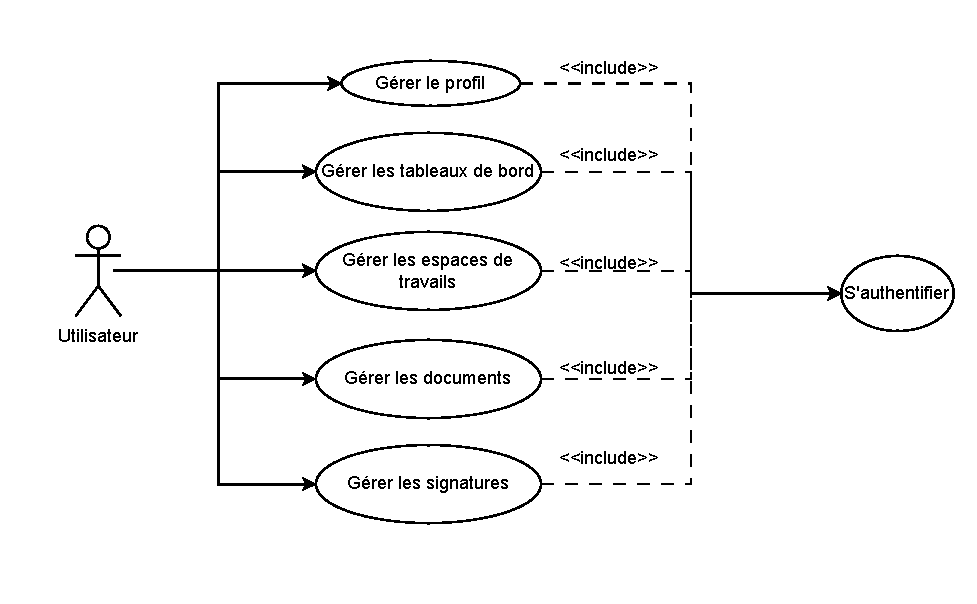
\includegraphics[width=0.6\textwidth]{useCaseGeneral}
\caption{Diagramme de cas d'utilisation global}
\end{figure}

\section{Le pilotage du projet par SCRUM}
Scrum est basé sur un ensemble de concepts permettant d'assurer une bonne gestion des projets : rôle, artefacts, sprint et réunion.

\subsection{Identification de l'équipe SCRUM}
L'équipe joue un rôle capital dans Scrum : elle permet d'optimiser la productivité et la
flexibilité.

Afin de parvenir à ces objectifs, elle doit s'auto organiser et être multi compétente. Elle doit également avoir un champ d'action suffisant pour la soutenir dans la réalisation de son travail
Dans le contexte de notre projet, on trouve :

\begin{itemize}
  \item \textbf{Product Owner} Quentin DEMARTHE
  \item \textbf{Scrum Master} Rabii MEJAI
  \item \textbf{Equipe de développement} : Mohamed Youssef CHLENDI, Raed CHARRAD
\end{itemize}